\section{Results}
\label{sec:results}

\subsection{Period-0 results}

Table~\ref{tab:t0} summarizes the experiment that uses only period~0. All ten runs produced a
feasible solution.

\begin{table}[h!]
\centering
\caption{Period 0 results over ten runs (limit: 1800\,s). SD is the sample standard deviation of MLU;
solver time, gap, and nodes are means.}
\label{tab:t0}
\renewcommand{\arraystretch}{1.1}
\footnotesize
\setlength{\tabcolsep}{4pt}
\begin{tabular}{@{}lrrrrrrrrrr@{}}
\toprule
\textbf{Inst.} & \textbf{$|V|$} & \textbf{$|A|$} & \textbf{$|D|$} & \textbf{Best} & \textbf{Mean} &
\textbf{SD} & \textbf{Solver (s)} & \textbf{Gap} & \textbf{Nodes} & \textbf{Cert.} \\
\midrule
A01 & 20 & 80 & 40 & 0.9294 & 0.9294 & 0 & 1.05 & 0 & 1.0 & 10/10 \\
A02 & 30 & 150 & 45 & 0.5486 & 0.5486 & 0 & 2.79 & 0 & 1.0 & 10/10 \\
A03 & 50 & 250 & 20 & 0.9435 & 0.9435 & 0 & 39.4 & 0 & 1.0 & 10/10 \\
A04 & 50 & 250 & 200 & 0.4591 & 0.4591 & 0 & 1744.0 & $1.12\times10^{-4}$ & 105.7 & 0/10 \\
A05 & 100 & 396 & 100 & 0.1155 & 0.1155 & 0 & 0.03 & 0 & 0.0 & 10/10 \\
A06 & 100 & 500 & 500 & 0.0986 & 0.0986 & 0 & 352.3 & 0 & 795.0 & 10/10 \\
A07 & 100 & 500 & 800 & 0.9080 & 0.9080 & 0 & 0.03 & 0 & 0.0 & 10/10 \\
A08 & 150 & 654 & 200 & 0.3189 & 0.3189 & 0 & 2.69 & 0 & 2.1 & 10/10 \\
A09 & 150 & 750 & 200 & 0.5054 & 0.5054 & 0 & 0.04 & 0 & 1.0 & 10/10 \\
A10 & 150 & 966 & 1000 & 0.0761 & 0.0761 & 0 & 1739.3 & 0.1020 & 272.6 & 0/10 \\
A11 & 200 & 1000 & 400 & 0.6555 & 0.6555 & 0 & 1741.0 & 0.0646 & 1.3 & 0/10 \\
A12 & 200 & 898 & 400 & 0.6401 & 0.6401 & 0 & 1299.3 & 0.0955 & 9.9 & 0/10 \\
A13 & 200 & 1000 & 2000 & 0.0389 & 0.0389 & 0 & 1741.5 & $9.99\times10^{-4}$ & 2690.6 & 0/10 \\
A14 & 250 & 1108 & 600 & 0.4240 & 0.4240 & 0 & 1745.2 & $1.43\times10^{-4}$ & 119.2 & 0/10 \\
A15 & 250 & 1250 & 600 & 0.8252 & 0.8252 & 0 & 0.04 & 0 & 0.0 & 10/10 \\
A16 & 250 & 1452 & 4800 & 0.0389 & 0.0393 & $2.8\times10^{-4}$ & 1787.0 & 0.0172 & 12398.5 & 0/10 \\
A17 & 300 & 1270 & 2000 & 0.4242 & 0.4242 & 0 & 0.05 & 0 & 0.0 & 10/10 \\
A18 & 300 & 1500 & 2000 & 0.6334 & 0.6334 & 0 & 0.04 & 0 & 0.0 & 10/10 \\
A19 & 300 & 1998 & 6000 & 0.0475 & 0.0483 & $4.5\times10^{-4}$ & 1774.2 & 0.0296 & 8516.1 & 0/10 \\
A20 & 400 & 2000 & 6000 & 0.9913 & 0.9913 & 0 & 0.09 & 0 & 0.0 & 10/10 \\
\bottomrule
\end{tabular}
\end{table}

Twelve instances are certified MLU-optimal in all ten runs. Some large instances require very little
solver time. For example, setA-20 has 400 vertices and 6000 demands, but its calls to
\texttt{optimize!} take only 0.09 seconds on average because the lower bound already matches the
feasible incumbent. This is not an end-to-end runtime: graph construction, pricing, and column
generation are excluded.

The remaining eight instances are not certified within the available time. However, the final gaps
for setA-04, setA-13, and setA-14 are below $10^{-3}$, so their reported solutions are close to the
corresponding lower bounds. In contrast, setA-10, setA-11, and setA-12 retain mean gaps of 10.20\%,
6.46\%, and 9.55\%, respectively. SetA-16 and setA-19 also show some variation in their feasible
objective values across the ten seeds; the best values found are 0.0389 and 0.0475, compared with the
displayed means of 0.0393 and 0.0483.

\subsection{Two-period results}

The two-period model is certified MLU-optimal in all ten runs for thirteen instances. SetA-03 has mixed
results: eight runs prove an optimum of 0.9435, while two runs reach 0.9444 before the time limit. The
other six instances without a complete certificate are setA-04, setA-10, setA-13, setA-14, setA-16,
and setA-19. Among them, setA-04 remains very close to its lower bound, with a mean gap of only
$1.61\times10^{-4}$. SetA-16 and setA-19 are much harder for the implemented method, ending with mean
gaps of 66.82\% and 55.86\%. These large gaps indicate weak certificates; they do not by themselves
show that the feasible solutions are poor.

\begin{table}[h!]
\centering
\caption{Joint two-period results over ten runs with the reconfiguration budget (limit: 3600\,s). SD
is the sample standard deviation of MLU; solver time, gap, and nodes are means.}
\label{tab:full}
\renewcommand{\arraystretch}{1.1}
\footnotesize
\setlength{\tabcolsep}{4pt}
\begin{tabular}{@{}lrrrrrrrrrr@{}}
\toprule
\textbf{Inst.} & \textbf{$|V|$} & \textbf{$|A|$} & \textbf{$|D|$} & \textbf{Best} & \textbf{Mean} &
\textbf{SD} & \textbf{Solver (s)} & \textbf{Gap} & \textbf{Nodes} & \textbf{Cert.} \\
\midrule
A01 & 20 & 80 & 40 & 0.9294 & 0.9294 & 0 & 14.6 & 0 & 1.0 & 10/10 \\
A02 & 30 & 150 & 45 & 0.9031 & 0.9031 & 0 & 152.7 & 0 & 1.0 & 10/10 \\
A03 & 50 & 250 & 20 & 0.9435 & 0.9437 & $3.7\times10^{-4}$ & 1430.5 & 0.0030 & 33.1 & 8/10 \\
A04 & 50 & 250 & 200 & 0.5812 & 0.5812 & $1.1\times10^{-7}$ & 3592.7 & $1.61\times10^{-4}$ & 1503.4 & 0/10 \\
A05 & 100 & 396 & 100 & 0.2050 & 0.2050 & 0 & 0.32 & 0 & 1.0 & 10/10 \\
A06 & 100 & 500 & 500 & 0.0986 & 0.0986 & 0 & 168.0 & 0 & 540.8 & 10/10 \\
A07 & 100 & 500 & 800 & 0.9080 & 0.9080 & 0 & 42.3 & 0 & 229.6 & 10/10 \\
A08 & 150 & 654 & 200 & 0.3189 & 0.3189 & 0 & 1.26 & 0 & 3.0 & 10/10 \\
A09 & 150 & 750 & 200 & 0.8497 & 0.8497 & 0 & 2.60 & 0 & 2.0 & 10/10 \\
A10 & 150 & 966 & 1000 & 0.0717 & 0.0733 & 0.0013 & 3594.1 & 0.0678 & 4947.0 & 0/10 \\
A11 & 200 & 1000 & 400 & 0.7858 & 0.7858 & 0 & 2.92 & 0 & 2.0 & 10/10 \\
A12 & 200 & 898 & 400 & 0.8799 & 0.8799 & 0 & 1.82 & 0 & 2.0 & 10/10 \\
A13 & 200 & 1000 & 2000 & 0.0415 & 0.0420 & $4.9\times10^{-4}$ & 3591.1 & 0.0288 & 7846.2 & 0/10 \\
A14 & 250 & 1108 & 600 & 0.5176 & 0.5176 & 0 & 3608.9 & 0.0197 & 17922.4 & 0/10 \\
A15 & 250 & 1250 & 600 & 0.8987 & 0.8987 & 0 & 5.61 & 0 & 1.0 & 10/10 \\
A16 & 250 & 1452 & 4800 & 0.1025 & 0.1369 & 0.0245 & 3594.2 & 0.6682 & 32238.2 & 0/10 \\
A17 & 300 & 1270 & 2000 & 0.4242 & 0.4242 & 0 & 50.5 & 0 & 1.0 & 10/10 \\
A18 & 300 & 1500 & 2000 & 1.0000 & 1.0000 & 0 & 32.8 & 0 & 0.0 & 10/10 \\
A19 & 300 & 1998 & 6000 & 0.0796 & 0.1096 & 0.0199 & 3542.7 & 0.5586 & 15254.0 & 0/10 \\
A20 & 400 & 2000 & 6000 & 0.9913 & 0.9913 & 0 & 401.9 & 0 & 2.0 & 10/10 \\
\bottomrule
\end{tabular}
\end{table}

\subsection{Comparison of the two experiments}

Figure~\ref{fig:mlu} makes the effect of adding period~1 easier to see. For setA-01, setA-06, setA-07,
setA-08, setA-17, and setA-20, the certified two-period optimum is equal to the period-0 optimum. In
these instances, the reconfiguration budget still allows routes whose peak utilization does not
increase. For several other certified cases, the second period raises the MLU substantially: from
0.5486 to 0.9031 on setA-02, from 0.1155 to 0.2050 on setA-05, from 0.5054 to 0.8497 on setA-09, and
from 0.6334 to 1.0000 on setA-18.

\begin{figure}[h!]
\centering
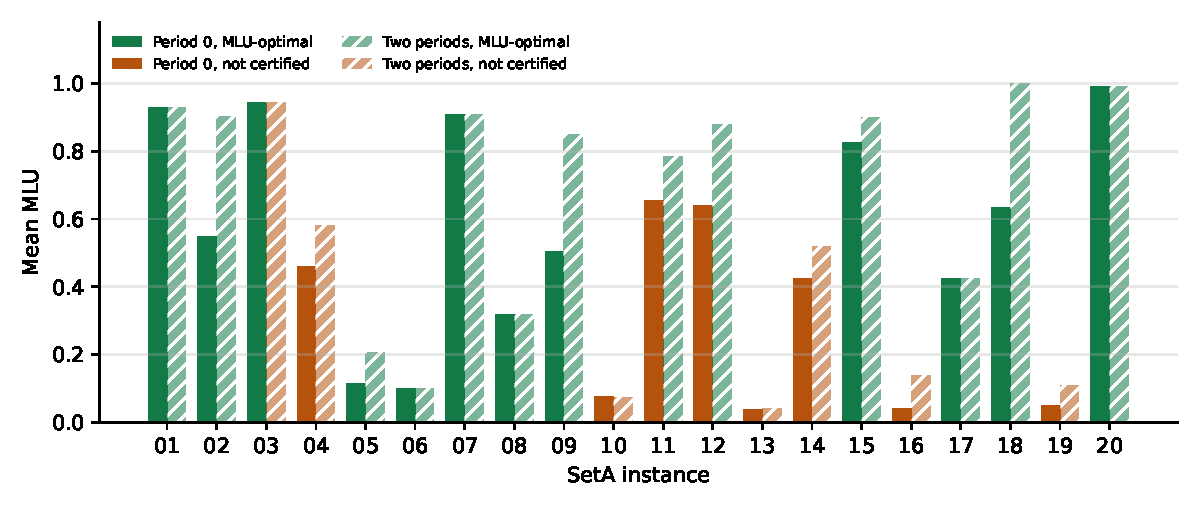
\includegraphics[width=\linewidth]{mlu_compare.pdf}
\caption{Mean MLU for period~0 (solid bars) and for the joint two-period model (hatched bars). Green
indicates that all ten runs are certified MLU-optimal; amber indicates that at least one run is not
certified.}
\label{fig:mlu}
\end{figure}

The two tables should be compared carefully when either row is not certified. For example, the mean
feasible MLU of setA-10 is lower in the two-period experiment than in the period-0 experiment. This
does not mean that adding a period improves the true optimum. Both rows are non-optimal search
results, and the longer two-period run simply found a better feasible period-0-compatible routing. The
same caution applies to comparisons involving setA-13, setA-16, and setA-19.
